\documentclass[10pt]{report}
\usepackage{/Users/bradenhoagland/latex/math}

\lhead{Braden Hoagland}
\chead{Topology}
\rhead{}

% make all mathcal symbols look different
\usepackage{dutchcal}

\begin{document}
\tableofcontents

%+-------------------+
%| +---------------+ |
%| |    Chapter    | |
%| +---------------+ |
%+-------------------+
% Topological Spaces


\chapter{Topological Spaces}

%%%%%%%%%%%%%%%%%%%%
% Topological Spaces
%%%%%%%%%%%%%%%%%%%%

\section{Topological Spaces}


\begin{defn}{Topology}{}
	Let $X$ be a set, then a \textbf{topology} on $X$ is a collection $\mathcal{T}$ of subsets of $X$ such that
	\begin{enumerate}
		\item $\varnothing, X \in \mathcal{T}$,
		\item $\bigcup_{\alpha\in \mathcal{J}}U_\alpha \in \mathcal{T}$, and
		\item $\bigcap_{i=1}^N U_i \in \mathcal{T}$.
	\end{enumerate}
	Elements of a topology are called \textbf{open sets}.
\end{defn}

\begin{ex}{Topological Spaces}{}
\begin{enumerate}
	\item ``Indiscrete" topology: $\mathcal{T}_i = \left\{ \varnothing, X \right\}$ 
	\item ``Discrete" topology: $\mathcal{T}_d =\{$all subsets of $X\}$
\end{enumerate}
\end{ex}

\begin{defn}{Finer/Coarser}{}
	Let $\mathcal{T},\mathcal{T}'$ be topologies on a set $X$, then $\mathcal{T}$ is \textbf{finer} than $\mathcal{T}'$ if $\mathcal{T}' \subset \mathcal{T}$. It is \textbf{strictly finer} if, in addition, $\mathcal{T}' \neq \mathcal{T}$.

	$\mathcal{T}$ is \textbf{coarser} than $\mathcal{T}'$ if $\mathcal{T} \subset \mathcal{T}'$. It is \textbf{strictly coarser} if, in addition, $\mathcal{T}' \neq \mathcal{T}$.
\end{defn}

From this we see that ``fine" is a notion of a large topology, and ``coarse" is a notion of a small topology.

\begin{ex}{Finite Complement Toplogy}{}
	Let $X$ be any set, then the \textbf{finite complement topology} is defined
	\[
		\mathcal{T}_f = \left\{ U \subset X \;|\; X-U \text{ is finite} \right\} \cup\left\{ \varnothing \right\},
	\] 
	where $X-U$ denotes the complement of $U$ in $X$, i.e. $X \backslash U$. Checking that this is a topology boils down to just using DeMorgan's Laws.
\end{ex}

%%%%%%%%%%%%%%%%%%%%
% Bases
%%%%%%%%%%%%%%%%%%%%

\section{Bases}

\begin{defn}{Basis}{}
Let $\mathcal{T}$ be a topoloy on $X$, and let $\mathcal{B} \subset \mathcal{T}$. Then $\mathcal{B}$ is a \textbf{basis} for $\mathcal{T}$ if every open set of $\mathcal{T}$ can be written as the union of elements of $\mathcal{B}$.
\end{defn}

\begin{prop}
\label{prop:basis-specific-top}
Let $\mathcal{T}$ be a topology on $X$, and let $\mathcal{B}$ be a collection of subsets of $X$. Then $\mathcal{B}$ is a basis for $\mathcal{T}$ if and only if
\begin{enumerate}
	\item $\mathcal{B}\subset \mathcal{T}$; and
	\item for each $U \in \mathcal{T}$ and $p \in U$, there is a $B \in \mathcal{B}$ such that $p \in B \subset U$.
\end{enumerate}
\end{prop}
\begin{proof}
	The forward direction follows from every open set of $\mathcal{T}$ being the union of elements of $\mathcal{B}$. For the backward direction, since $p \in B_p \subset U$ for all $p \in U$, we have $U = \bigcup_{p\in U}B_p$, so every open set of $\mathcal{T}$ is the union of elements of $\mathcal{B}$.
\end{proof}

\begin{figure}[H]
	\centering
	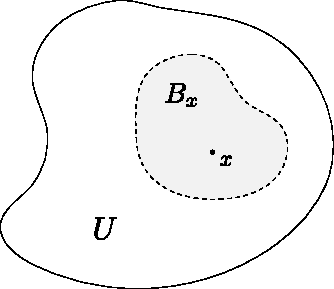
\includegraphics[scale=0.8]{fig/gen-top.pdf}
	\caption{For any $U \in \mathcal{T}$, each $x \in U$ lies in some $B_x \in \mathcal{B}$ for $B_x \subset U$.}
\end{figure}


Not every set of subsets of $X$ will generate a topology, so we need conditions for a collection $\mathcal{B}$ to be a basis for \textit{any} topology.

\begin{prop}
\label{prop:basis-for-any-top}
Let $\mathcal{B}$ be a collection of subsets of $X$. Then $\mathcal{B}$ generates a topology if and only if
\begin{enumerate}
	\item for each $x \in X$, there is a $B \in \mathcal{B}$ containing $x$; and
	\item given $B_1,B_2 \in \mathcal{B}$ and $x \in B_1 \cap B_2$, there is a $B_3 \in \mathcal{B}$ such that $x \in B_3 \subset B_1 \cap B_2$.
\end{enumerate}
\end{prop}
\begin{proof}
	\textbf{Forward:} (1) $X$ must be open, so $X$ is the union of elements of $\mathcal{B}$, so any $x \in X$ must lie in at least one of them. (2) Since $B_1$ and $B_2$ are both open in the topology generated by $\mathcal{B}$, their intersection is, as well. Then since $\mathcal{B}$ is a basis for this topology, we can find a satisfactory $B_3$.

	\textbf{Backward:} The topology generated by a set $\mathcal{B}$ is the collection of all unions of elements of $\mathcal{B}$. It is clear that $\varnothing$ is in it, and condition (1) implies that $X$ is, as well. Arbitrary unions are in the topology by definition. Induction on condition (2) shows that the topology also contains finite intersections.
\end{proof}

\begin{figure}[H]
	\centering
	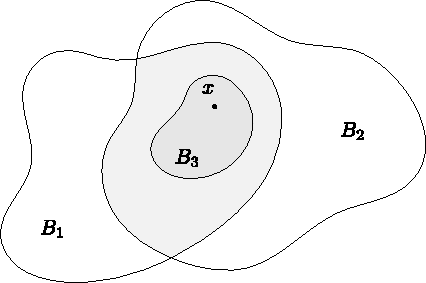
\includegraphics[scale=1]{fig/basis.pdf}
	\caption{Condition $(2)$ in Proposition \ref{prop:basis-for-any-top}.}
\end{figure}

Condition $(1)$ in the above proposition is saying that $X$ is the union of all elements of $\mathcal{B}$. Condition $(2)$ is used to ensure that finite intersections of open elements remain open.

Additionally, note that since $\mathcal{B}$ exists independently from any topology, it doesn't make sense to describe its members as ``open" until after we've generated a topology from it. Once we've done so, though, it should be clear that every basis element is open in the generated topology.

We can also get a notion of how relatively fine or coarse a topology is by using its basis.

\begin{prop}
	Let $\mathcal{B}, \mathcal{B}'$ be bases for the topologies $\mathcal{T},\mathcal{T}'$ on $X$, respectively. Then $\mathcal{T}'$ is finer than $\mathcal{T}$ if and only if for all $B \in \mathcal{B}$ and $x \in B$, there is a $B' \in \mathcal{B}'$ such that $x \in B' \subset \mathcal{B}$.
\end{prop}
\begin{proof}
	First we show the backward implication. Let $U \in \mathcal{T}$, and let $x \in U$. Since $\mathcal{B}$ generates $\mathcal{T}$, there is a $B \subset \mathcal{B}$ such that $x \in B \subset U$. By assumption, there is then a $B' \in \mathcal{B}'$ such that $x \in B' \subset B \subset U$. Thus $U \in \mathcal{T}'$, so $\mathcal{T}'$ is finer than $\mathcal{T}$.

	Now we show the forward implication. Let $B \in \mathcal{B}$, and let $x \in B$, then $B \in \mathcal{T}$. By assmption, $\mathcal{T} \subset \mathcal{T}'$, so $B \in \mathcal{T}'$ as well. Then by thedefinition of a generated topology, there is a $B' \subset \mathcal{B}'$ such that $x \in B' \subset B$.
\end{proof}

\begin{defn}{Topologies on $\mathbb{R}$}{}
If $\mathcal{B}$ is the collection of all open intervals of the real line, the topology generated by $\mathcal{B}$ is the \textbf{standard topology} on the real line.

If $\mathcal{B}$ is the collection of half-open intervals of the form $[a,b)$, it generates the \textbf{lower limit topology} on $\mathbb{R}$. When $\mathbb{R}$ is given the lower limit topology, we denote it by $\mathbb{R}_l$.

Let $K$ denote the set of all numbers of the form $1/n$ for $n \in \mathbb{Z}_+$, and let $\mathcal{B}$ be the collection of all open intervals $(a,b)$ along with all sets of the form $(a,b) - K$. Then $\mathcal{B}$ generates the \textbf{K-topology} on $\mathbb{R}$. When $\mathbb{R}$ is given this topology, we denote it by $\mathbb{R}_K$.
\end{defn}

\begin{prop}
	The topologies of $\mathbb{R}_l$ and $\mathbb{R}_K$ are strictly finer than the standard topology on $\mathbb{R}$, but are not comparable with each other.
\end{prop}
\begin{proof}
	Let $\mathcal{T}$, $\mathcal{T}'$, and $\mathcal{T}''$ be the topologies of $\mathbb{R}$, $\mathbb{R}_l$, and $\mathbb{R}_K$, respectively. Given a basis element $(a,b)$ of $\mathcal{T}$ and $x \in (a,b)$, the basis element $[x,b)$ of $\mathcal{T}'$ contains $x$ and lies in $(a,b)$. However, given the basis element $[x,d)$ of $\mathcal{T}'$, there is no open interval that contains $x$ and lies in $[x,d)$. Thus $\mathcal{T}'$ is strictly finer than $\mathcal{T}$.

	Similarly, given a basis element $(a,b)$ of $\mathcal{T}$ and $x \in (a,b)$, this same interval is a basis element for $\mathcal{T}''$ that contains $x$. However, given the basis element $B=(-1,1) - K$ for $\mathcal{T}''$ and the point $0 \in B$, there is no open interval that contains $0$ and lies in $B$ (since $\mathbb{Q}$ is dense in $\mathbb{R}$). Thus $\mathcal{T}''$ is strictly finer than $\mathcal{T}$.

	{\color{red}Show $\mathcal{T}'$ and $\mathcal{T}''$ aren't comparable.}
\end{proof}

%%%%%%%%%%%%%%%%%%%%
% Subbases
%%%%%%%%%%%%%%%%%%%%

\section{Subbases}

\begin{defn}{Subbasis}{}
	A \textbf{subbasis} $\mathcal{S}$ for a topology $\mathcal{T}$ on $X$ is a collection of subsets of $X$ whose finite intersections form a basis for $\mathcal{T}$.
\end{defn}

Subbases are easier to construct than bases, but the construction of a topology from a subbasis involves an extra step, namely the finite intersections. What we are doing is creating a basis $\mathcal{B}$ from $\mathcal{S}$ by taking finite intersections of the subbasis elements. Then we are taking $\mathcal{B}$ and constructing $\mathcal{T}$ by taking arbitrary unions, as is usual.

\begin{figure}[H]
	\centering
	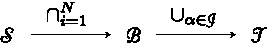
\includegraphics[scale=1]{fig/subbasis-to-topology.pdf}
	\caption{The process for constructing a topology using a subbasis $\mathcal{S}$.}
\end{figure}

{\color{red}Subbasis is smallest set contained in topology or something like that?}

\begin{prop}
Let $\mathcal{T}$ be a topology on $X$, and let $\mathcal{S}$ be a collection of subsets of $X$. Then $\mathcal{S}$ is a subbasis for $\mathcal{T}$ if and only if
\begin{enumerate}
	\item $\mathcal{S} \subset \mathcal{T}$; and
	\item for each $U \in \mathcal{T}$ and $p \in U$, there is a finite intersection $\bigcap_{i=1}^n S_i$ of elements of $\mathcal{S}$ such that $p \in \bigcap_{i=1}^n S_i \subset U$.
\end{enumerate}
\end{prop}
\begin{proof}
	This follows from Proposition \ref{prop:basis-specific-top} (the analogue of this proposition for bases). When proving both directions, there's just an extra step to go from a genric basis element to a finite intersection of elements of $\mathcal{S}$.
\end{proof}

Just as with bases, we have a condition for when an arbitrary collection of subsets of $X$ can be a valid subbasis.

\begin{prop}
Let $\mathcal{S}$ be a collection of subsets of $X$. Then $\mathcal{S}$ generates a topology if and only if every point of $X$ is in some element of $\mathcal{S}$.
\end{prop}
\begin{proof}
{\color{red}Sketch.}
\end{proof}


%%%%%%%%%%%%%%%%%%%%
% The Order Topology
%%%%%%%%%%%%%%%%%%%%

\section{The Order Topology}

\begin{defn}{Total Order}{}
A binary relation $\leq$ is a total order on a set $X$ if
 \begin{enumerate}
	\item $a \leq b, b \leq a \implies a=b$,
	\item $a\leq b, b\leq c \implies a \leq c$, and
	\item $a \leq b$ or $b \leq a$.
\end{enumerate}
\end{defn}

A totally ordered set $X$ can be divided into intervals of the form $(a,b)$, $(a,b]$, $[a,b)$, and $[a,b]$. Note that even though this is reminiscent of the real number line, this is for any arbitrary ordered set.

\begin{defn}{The Order Topology}{}
Let $X$ be a totally ordered set with more than one element, and let $\mathcal{B}$ be a collection of
\begin{enumerate}
	\item All open intervals $(a,b)$ in $X$,
	\item All half-open intervals $[a_0,b)$, where $a_0$ is the smallest element of $X$, and
	\item All intervals of the form $(a,b_0]$, where $b_0$ is the largest element of $X$.
\end{enumerate}
If $X$ has no smallest element there are no sets of type $(2)$, and if $X$ has no largest elemtn, there are no sets of type $(3)$. Then $\mathcal{B}$ is a basis for the \textbf{order topology} on $X$.
\end{defn}

\begin{ex}{}{}
The standard topology on $\mathbb{R}$, as defined in the previous section, is just the order topology derived from the usual order on $\mathbb{R}$.
\end{ex}

\begin{defn}{Ray}{}
	Let $a$ be an element of an ordered set $X$, then the \textbf{rays} of $X$ determined by $a$ are the subsets $(a,+\infty)$, $(-\infty,a)$, $[a,+\infty)$, and $(-\infty,a]$. The first two are \textbf{open rays} and the latter two are \textbf{closed rays}. 
\end{defn}

Based on the name, we expect open rays to be open sets in the order topology, and so they are. Consider $(a,\infty)$. If $X$ has a largest element $b_0$, then $(a,\infty)=(a,b_0]$, which is in the topology. If $X$ has no largest element, then $(a,\infty) = \bigcup_{x>a}(a,x)$, so it is open. The argument is similar for $(-\infty,a)$.

In fact, the open rays form a subbasis for the order topology on $X$. Since the open rays are open in the order topology, the topology they generate is contained in the order topology. On the other hand, every basis element for the order topology is a finite intersection of open rays. The interval $(a,b)$ is the intersection of $(-\infty,b)$ and $(a,\infty)$. If $[a_0,b)$ or $(a,b_0]$ exist, they are themselves open rays. Thus the topology generated by the open rays contains the order topology.


%%%%%%%%%%%%%%%%%%%%
% The (2D) Product Topology
%%%%%%%%%%%%%%%%%%%%

\section{The (2D) Product Topology}

{\color{red}Move general subspace stuff in here, up to but not including the stuff about Hausdorff, etc.}

\begin{defn}{Product Topology}{}
If $X$ and $Y$ are topological spaces, then the \textbf{product topology} on $X \times Y$ is the topology having as basis the collection $\mathcal{B}$ of all sets of the form $U \times V$, where $ U$ is a open subset of $X$ and $V$ is an open susbet of $Y$.
\end{defn}

Since $X \times Y$ is itself a basis element, the first condition for a basis is trivial. Note that \[
	(U_1 \times V_1) \cap (U_2 \times V_2) = (U_1 \cap U_2) \times (V_1 \cap V_2).
\] Since each of these is a finite intersection of open sets, they are themselves open. Thus the intersection is itself a basis element, and the second condition for a basis is satisfied.


\begin{thrm}{}{}
If $\mathcal{B}$ is a basis for the topology of $X$ and $\mathcal{C}$ is a basis for the topology of $Y$, then the collection
\[
\mathcal{D}=\left\{ B\times C \;|\; B \in \mathcal{B}, C \in \mathcal{C} \right\}
\] is a basis for the topology of $X \times Y$.
\end{thrm}
\begin{proof}
	Given an open set $W$ of $X \times Y$ and $x \times y \in W$, by definition of the product topology there is a basis element $U \times V$ such that $x \times y \in U \times V \subset W$. Since $\mathcal{B}$ and $\mathcal{C}$ are bases for $X$ and $Y$, respectively, we can choose an element $B\in\mathcal{B}$ such that $x \in B \subset U$ and an element $C \in \mathcal{C}$ such that $y \in C \subset V$. Then $x \times y \in B \times C \subset W$. Since $B \times C \in \mathcal{D}$, we have that $\mathcal{D}$ is a basis for $X \times Y$. {\color{red}Redo.}
\end{proof}

We can also express the product topology in terms of subbases, but we must first define projections.

\begin{defn}{Projection}{}
Let $\pi_1: X \times Y \to X$ be defined by
\[
	\pi_1(x,y) = x,
\] and let $\pi_2:X\times Y \to Y$ be defined by
\[
	\pi_2(x,y)=y,
\] then the maps $\pi_1$ and $\pi_2$ are called the \textbf{projections} of $X \times Y$ onto its first and second factors, respectively.
\end{defn}

Note that $\pi_1$ and $\pi_2$ are surjective (unless $X$ or $Y$ is empty, in which case $X \times Y$ is empty, but this is a meaningless case).

If $U$ is an open subset of $X$, then $\pi_1^{-1}(U)=U \times Y$, which is open in $X \times Y$. Similarly, if $V$ is open in $Y$, then $\pi_2^{-1}(V) = X \times V$, which is open in $X \times Y$ as well. The intersection of these two sets is $U \times V$, which leads to the following theorem.

\begin{figure}[H]
	\centering
	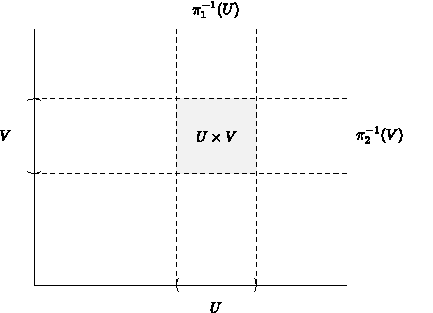
\includegraphics[scale=1.5]{fig/product-open.pdf}
	\caption{The open set in $X \times Y$ formed by the intersection of the preimages of the projections onto open sets $U \subset X$ and $V \subset Y$.}
\end{figure}


\begin{thrm}{}{}
The collection
\[
	\mathcal{S}=\left\{ \pi_1^{-1}(U) \;|\; U \text{ open in } X \right\} \cup \left\{ \pi_2^{-1}(V) \;|\; V \text{ open in } Y \right\}
\] is a subbasis for the product topology on $X \times Y$.
\end{thrm}
\begin{proof}
	Let $\mathcal{T}$ denote the product topology on $X \times Y$, and let $\mathcal{T}'$ be the topology generated by $\mathcal{S}$. Every element of $\mathcal{S}$ is in $\mathcal{T}$, so arbitrary unions of finite intersections of elements of $\mathcal{S}$ are also in $\mathcal{T}$. Thus $\mathcal{T}' \subset \mathcal{T}$. On the other hand, every basis element $U \times V$ for the topology $\mathcal{T}$ is a finite inersectino of elements of $\mathcal{S}$, since
	\[
		U \times V = \pi_1^{-1}(U) \cap \pi_2^{-1}(V).
	\] Then $U \times V \in \mathcal{T}'$, so $\mathcal{T}\subset \mathcal{T}'$. Thus $\mathcal{T}=\mathcal{T}'$.
\end{proof}

%%%%%%%%%%%%%%%%%%%%
% The Subspace Topology
%%%%%%%%%%%%%%%%%%%%

\section{The Subspace Topology}

\begin{defn}{Subspace Topology}{}
	Let $(X,\mathcal{T})$ be a topological space. If $Y \subset X$, then
	\[
	\mathcal{T}_Y = \left\{ Y \cap U \;|\; U \in \mathcal{T} \right\}
	\] is the \textbf{subspace topology} on $Y$. With this topology, $Y$ is called a \textbf{subspace} of $X$.
\end{defn}

\begin{prop}
	$\mathcal{T}_Y$ is a topology on $Y$.
\end{prop}
\begin{proof}
	$\varnothing \cap Y = \varnothing \in \mathcal{T}_Y$. Additionally, $Y \subset X$ implies $Y = Y \cap X$, so $Y \in \mathcal{T}_Y$. Arbitrary unions are open since
	\[
		\bigcup_{\alpha\in\mathcal{J}}(U_\alpha \cap Y) = \bigg( \bigcup_{\alpha\in\mathcal{J}}U_\alpha \bigg) \cap Y \in \mathcal{T}_Y.
	\] 
	Finite intersections are also open since
	\[
		\bigcap_{i=1}^N (U_i \cap Y) = \bigg( \bigcap_{i=1}^N U_i \bigg) \cap Y \in \mathcal{T}_Y.
	\] 
\end{proof}

\begin{prop}
Let $\mathcal{B}$ be a basis for the topology of $X$, then \[\mathcal{B}_Y \doteq \left\{ B \cap Y \;|\; B \in \mathcal{B} \right\}\] is a basis for the subspace topology on $Y$.
\end{prop}
\begin{proof}
	Let $y \in U \cap Y$, where $U$ is open in $X$. There exists $B \in \mathcal{B}$ such that $y \in B \subset U$, so $y \in B \cap Y \subset U \cap Y$.
\end{proof}

\begin{prop}
	Let $Y$ be a subspace of $X$, and let $U$ be open in $Y$ and $Y$ be open in $X$. Then $U$ is open in $X$.
\end{prop}
\begin{proof}
	$U$ is open in $Y$, so $U=Y \cap V$ for some $V$ open in $X$. Both sets $Y$ and $V$ are open in $X$, so their intersection $U$ must be as well.
\end{proof}

\begin{thrm}{}{}
Let $A$ be a subspace of $X$ and $B$ be a subspace of $Y$, then the product topology on $A \times B$ is the same as the topology $A \times B$ inherits as a subspace of $X \times Y$.
\end{thrm}
\begin{proof}
	$U \times V$ is the general basis element for $X \times Y$, where $U$ is open in $X$ and $V$ is open in $Y$. Thus $(U \times V) \cap (A \times B) = (U \cap A) \times (V \cap B)$ is the general basis element for the subspace topology on $A \times B$.

	Since $U \cap A$ and $V \cap B$ are the general open sets for the supspace topology on $A$ and $B$, respectively, $(U \cap A) \times (V \cap B)$ is the general basis element for the product topology on $A \times B$.

	This shows that the two topologies have the same bases, so the topologies themselves must be the same.
\end{proof}

This equivalence of topologies holds for the product topology, but not in general for the order topology, however.

\begin{ex}{}{}
	Let $Y=[0,1] \cap \left\{ 2 \right\}$ be a subset of $\mathbb{R}$. $\left\{ 2 \right\}$ is open in the subspace topology since $(3/2, 5/2) \cap Y = \left\{ 2 \right\}$, but $\left\{ 2 \right\}$ is not open in the order topology since no sets of the form $(a,b)$, $(a,b]$, or $[a,b)$ contain $\left\{ 2 \right\}$ without also containing points not in $Y$.
\end{ex}

It \textit{is} possible to have equivalence with the ordered topology, though. We can define a condition in which this equivalence holds, but we'll need another definition first.

\begin{defn}{Convex}{}
	Let $X$ be an ordered set, then $Y \subset X$ is \textbf{convex} in $X$ if for all pairs $a$ and $b$ in $Y$ such that $a<b$, the interval $(a,b) \subset X$ also lies in $Y$.
\end{defn}

Note that intervals and rays in $X$ are convex in $X$.

\begin{thrm}{}{}
Let $X$ be an ordered set in the order topology, and let $Y \subset X$ be convex in $X$. Then the order topology on $Y$ is the same as the topology $Y$ inherits as a subspace of $X$.
\end{thrm}
\begin{proof}
	Consider $(a,\infty) \subset X$. If $a \in Y$, then $(a,\infty) \cap Y = \left\{ x \;|\; x\in Y, x > a \right\}$. This is an open ray of $Y$. If $a \not\in Y$, then $a$ is either a lower bound or upper bound of $Y$. If $a$ is a lower bound of $Y$, then $(a,\infty) \cap Y = Y$. If $a$ is an upper bound of $Y$, then $(a,\infty) \cap Y = \varnothing$.

	Similarly, $(-\infty,a) \cap Y$ is either $\varnothing$, $Y$, or an open ray of $Y$.

	Since $(a,\infty)\cap Y$ and $(-\infty,a) \cap Y$ form a subbasis for the subspace topology on $Y$, and since each is open in the order topology, the order topology contains the subspace topology.

	Any open ray of $Y$ is the intersection of open rays of $X$ with $Y$, so it is open in the subspace topology on $Y$. Since the open rays of $Y$ are a subbasis for the order topology on $Y$, the order topology is contained in the subspace topology. Thus the order topology is the same as the subspace topology in this case.
\end{proof}

From here on out, assume that if $X$ is an ordered set in the order topology and $Y \subset X$, then $Y$ has the subspace topology. If $Y$ is convex in $X$, this is the same as the order topology on $Y$, otherwise it might not be.

%%%%%%%%%%%%%%%%%%%%
% Closed Sets and Limit Points
%%%%%%%%%%%%%%%%%%%%

\section{Closed Sets and Limit Points}

\begin{defn}{Closed Set}{}
	A set $A \subset (X, \mathcal{T})$ is closed if $X-A$ is open in $X$.
\end{defn}

\begin{thrm}{}{}
	Let $(X, \mathcal{T})$ be a topological space, and let $F$ denote a closed set of $X$, then
	\begin{enumerate}
		\item $\varnothing$ and $X$ are closed,
		\item $\bigcap_{\alpha\in\mathcal{J}}F_\alpha$ is closed, and
		\item $\bigcup_{i=1}^N F_i$ is closed.
	\end{enumerate}
\end{thrm}
The proof of this is a straightforward application of DeMorgan's Laws.

\begin{prop}
	\label{closed-isct}
Let $Y$ be a subspace of $X$. Then $A$ is closed in $Y$ if and only if it is equal to the intersection of a closed set of $X$ with $Y$.
\end{prop}
\begin{proof}
	First we show the forward implication. Assume $A$ is closed in $Y$, then $Y-A$ is open in $Y$, so be definition $Y-A=U \cap Y$ for some $U$ open in $X$. $X-U$ is closed in $X$, and $A = Y \cap (X-U)$, so $A$ is the intersection of a closed set of $X$ with $Y$.

	Now we show the backward implication. Assume $A = C \cap Y$ for $C$ closed in $X$. Then $X-C$ is open in $X$, so $(X-C) \cap Y$ is open in $Y$ by the definition of the subspace topology. But $(X-C) \cap Y = Y-A$, so $Y-A$ is open in $Y$. Thus $A$ is closed in $Y$.
\end{proof}

\begin{prop}
Let $Y$ be a subspace of $X$. If $A$ is closed in $Y$ and $Y$ is closed in $X$, then $A$ is closed in $X$.
\end{prop}
\begin{proof}
	$A = F \cap Y$ for some $F$ closed in $X$. $A$ is then the intersection of closed sets of $X$, so it is itself closed in $X$.
\end{proof}

\begin{figure}[H]
	\centering
	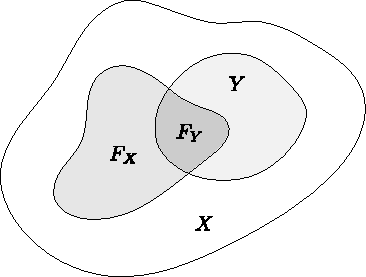
\includegraphics[scale=1]{fig/closed-isct.pdf}
	\caption{A set $F_Y$ closed in $Y$, where $F_Y = Y \cap F_X$ for $F_X$ closed in $X$.}
\end{figure}

\begin{defn}{Interior of a Set}{}
	The \textbf{interior} of a set $A$, denoted $A^o$, is the union of all open sets contained in $A$.
\end{defn}

\begin{defn}{Closure of a Set}{}
	The \textbf{closure} of a set $A$, denoted $\overline{A}$ is the intersection of all closed sets containing $A$.
\end{defn}

The closure of a set is clearly closed, and the interior of a set is clearly open. It is also clear that if $A$ is open, then $A^o = A$, and if $A$ is closed, then $\overline{A}=A$. We also have the obvious relation $A^o \subset A \subset \overline{A}$.

We have to be careful when describing closures. Given a subspace $Y$ of $X$, the closure of $A$ in $X$ is generally not the same as the closure of $A$ in $Y$. In this case, we use $\overline{A}$ to denote the closure of $A$ in $X$ (the overall space). We relate this to the closure of $A$ in $Y$ (the subspace) with the following proposition.

\begin{prop}
	Let $Y$ be a subspace of $X$, and let $A \subset Y$. Denote the closure of $A$ in $X$ by $\overline{A}$. Then the closure of $A$ in $Y$ is equal to $\overline{A} \cap Y$.
\end{prop}
\begin{proof}
	Let $B$ denote the closure of $A$ in $Y$. $\overline{A}$ is closed in $X$, so by Proposition \ref{closed-isct}, $\overline{A} \cap Y$ is closed in $Y$. Since $\overline{A} \cap Y$ contains $A$, and since by definition $B$ is the intersection of all closed subsets of $Y$ containing $A$, we have $B \subset \overline{A}\cap Y$.

	On the other hand, we know $B$ is closed in $Y$. Again by Proposition \ref{closed-isct}, $B = C \cap Y$ for some $C$ closed in $X$. Then $C$ is a closed set of $X$ containing $A$. Since $\overline{A}$ is the intersection of all such closed sets, we have $\overline{A} \subset C$, so $(\overline{A} \cap Y) \subset (C \cap Y) = B$.
\end{proof}

\begin{defn}{Neighborhood}{}
A \textbf{neighborhood} of a point $X$ is an open set containing $x$.
\end{defn}

\begin{thrm}{}{nhood-closure}
Let $A$ be a subset of a topological space $X$, then
\begin{enumerate}
	\item $x \in \overline{A}$ if and only if every neighborhood of $x$ intersects $A$, and
	\item Supposing the topology of $X$ is given by a basis, then $x \in \overline{A}$ if and only if every basis element $B$ containing $x$ intersects $A$.
\end{enumerate}
\end{thrm}
\begin{proof}
	\begin{enumerate}
		\item We'll prove the contrapositive: $x \not\in \overline{A}$ if and only if there exists an open neighborhood of $x$ that does not intersect $A$. We will first show the forward implication. Assume $x \not\in \overline{A}$, then $U = X-\overline{A}$ is open, contains $x$, and does not intersect $A$.

			Now we show the backward implication. Assume there exists an open neighborhood $U$ of $x$ that does not intersect $A$, then $X-U$ is a closed set containing $A$. By the definition of $\overline{A}$, $X-U$ must contain $\overline{A}$. Thus $x \not\in \overline{A}$.

		\item First we show the forward implication. By (1) we know if $x \in  \overline{A}$, then every open neighborhood of $x$ intersects $A$. Since basis elements are open, this implies that every basis element containing $x$ intersects $A$.

			Now we show the backward implication. Assume every basis element containing $x$ intersects $A$. Since every open neighborhood $U$ of $x$ contains some basis element, every such $U$ also intersects $A$. Again by (1), this implies $x \in \overline{A}$.
	\end{enumerate}
\end{proof}

\begin{defn}{Limit Point}{}
	Let $A \subset (X,\mathcal{T})$, then $x \in X$ is a \textbf{limit point}/cluster point/accumulation point of $A$ if every open neighborhood of $x$ intersects $A$ at some point \textit{other than $x$ }.

	Equivalently, $x$ belongs to the closure of $A - \left\{ x \right\}$. Note that $x$ need not lie in $A$.
\end{defn}

\begin{thrm}{}{}
	Let $A \subset (X,\mathcal{T})$, and denote the set of limit points of $A$ by $A'$. Then $\overline{A}=A \cup A'$.
\end{thrm}
\begin{proof}
	First we show $A' \cup A \subset \overline{A} $. Let $x \in A'$, then every open neighborhood of $x$ intersects $A$ (at a point other than $x$). Thus by Theorem \ref{thrm:nhood-closure}, $x \in \overline{A}$, so $A' \subset  \overline{A}$. Since $A \subset \overline{A}$ by definition, we have $A \subset A' \subset \overline{A}$.

	Now we show $\overline{A} \subset A' \cup A$. Let $x \in \overline{A}$. If $x \in A$, then this is trivial, so assume $x \not\in A$. Since $x \in \overline{A}$, every neighborhood of $x$ intersects $A$. Since $x \not\in A$, this must be at a point other than $x$. Thus $x \in A'\subset A' \cup A$, so $\overline{A} \subset A' \cup A$.
\end{proof}

\begin{cor}
	A subset of a topological space is closed if and only if it contains all its limit points.
\end{cor}
\begin{proof}
	Let $A \subset (X, \mathcal{T})$. Then $A$ is closed if and only if $A = \overline{A} = A \cup A'$, and $A = A \cup A'$ if and only if $A' \subset A$.
\end{proof}


%+-------------------+
%| +---------------+ |
%| |    Chapter    | |
%| +---------------+ |
%+-------------------+
% Separation Properties

\chapter{Separation Properties}


%%%%%%%%%%%%%%%%%%%%
% The Separation Axioms
%%%%%%%%%%%%%%%%%%%%

\section{The Separation Axioms}

Turns out that separating points yields some nice properties of topological spaces. Who'da thunk?

{\color{red}Stuff about $T_1$-$T_4$. Theorems about how they're related.}

\begin{figure}[H]
	\centering
	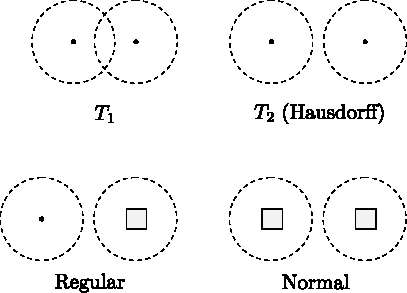
\includegraphics[scale=1]{fig/separation.pdf}
	\caption{The four main types of separation.}
\end{figure}

\begin{prop}
	Let $X$ be $T_1$, and let $A$ be a subset of $X$. Then $x$ is a limit point of $A$ if and only if every neighborhood of $x$ contains infinitely many points of $A$.
\end{prop}
\begin{proof}
	\textbf{Backward:} Every neighborhood of $x$ intersects $A$ at infinitely many points, so it they surely all intersect $A$ at a point other than $x$. Thus $x$ is a limit point.

	\textbf{Forward:} Let $x$ be a limit point of $A$, and suppose some neighborhood $U$ of $x$ intersects $A$ at only finitely many points. Let $\left\{ x_1,\dots,x_m \right\} = U \cap (A-\left\{ x \right\})$, then $X - \left\{ x_1,\dots,x_m \right\}$ is open in $X$ since $X$ satisfies the $T_1$ axiom. Then $U \cap (X - \left\{ x_1,\dots,x_m \right\})$ is a neighborhood of $x$ that doesn't intersect $A - \left\{ x \right\}$ at all. This contradicts $x$ being a limit point of $A$, so every neighborhood of $x$ must intersect $A$ at infinitely many points.
\end{proof}

\begin{prop}
	A space is $T_1$ if and only if all single points are closed.
\end{prop}
\begin{proof}
	\textbf{Forward:} Suppose $X$ is $T_1$, then fix $x \in X$. Then for $y \in X- \left\{ x \right\}$, there is an open $U_{y}$ such that $y \in U_y \subset X - \left\{ x \right\}$, so $X - \left\{ x \right\} = \bigcup_{y}U_y$. Then $X-\left\{ x \right\}$ is open so $\left\{ x \right\}$ is closed.

	\textbf{Backward:} Suppose all single points in $X$ are closed. Fix $x,y \in X$, then $X-\left\{ x \right\}$ and $X-\left\{ y \right\}$ are the open sets we need to show that $X$ is $T_1$.
\end{proof}

\begin{cor}
	A space is $T_1$ if and only if all finite point sets are closed.
\end{cor}
\begin{proof}
	{\color{red}Do I even need one? Kinda obvious.}
\end{proof}

%%%%%%%%%%%%%%%%%%%%
% Hausdorff Spaces
%%%%%%%%%%%%%%%%%%%%

\section{Hausdorff Spaces}

In a Hausdorff space, any two distinct points can be separated by disjoint open sets.

\begin{figure}[H]
	\centering
	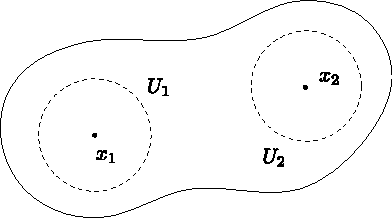
\includegraphics[scale=1]{fig/hausdorff.pdf}
	\caption{Two points in a Hausdorff space.}
\end{figure}


\begin{prop}
	Every finite set in a Hausdorff space is closed.
\end{prop}
\begin{proof}
	{\color{red}This follows from $T_1$, so move this proof up to $T_1$ proposition.}

	Let $X$ be a Hausdorff space. It suffices to show the arbitrary single point set $\left\{ x_0 \right\}$ is closed, as any finite set is the finite union of single points. Let $x \in X$ such that $x \neq x_0$, then $x$ and $x_0$ have disjoint neighborhoods. Thus $x$'s neighborhood does not intersect $\left\{ x_0 \right\}$, so $x$ is not in the closure of $\left\{ x_0 \right\}$. Since $x$ was arbitrary, the closure of $\left\{ x_0 \right\}$ is just $\left\{ x_0 \right\}$ itself, so it is closed.
\end{proof}

\begin{prop}
	Let $X$ be a Hausdorff space, then a sequence of points in $X$ converges to at most one point in $X$.
\end{prop}
\begin{proof}
	Suppose $\left\{ x_n \right\} \subset X$ such that $x_n \to x \in X$. If $y \neq x$, then since $X$ is Hausdorff we can find disjoint open neighborhoods $U$ and $V$of $x$ and $y$, respectively. The set $U$ contains all but finitely many of the points in $\left\{ x_n \right\}$, so $V$ can only contain finitely many of the points in $\left\{ x_n \right\}$. Thus $x_n$ cannot converge to $y$.
\end{proof}

\begin{prop}
	Every simply ordered set is Hausdorff in the order topology.
\end{prop}
\begin{proof}
	{\color{red}Do this.}
\end{proof}

\begin{prop}
	The product of two Hausdorff spaces is a Hausdorff space.
\end{prop}
\begin{proof}
	{\color{red}Do this.}
\end{proof}

\begin{prop}
	A subspace of a Hausdorff space is Hausdorff.
\end{prop}
\begin{proof}
	Suppose $X$ is Hausdorff and that $Y$ is a subspace of $X$ with distinct points $u$ and $v$. Then $u$ and $v$ are also distinct points of $X$, so by the regularity of $X$, they are separated by disjoint open sets $U$ and $V$ in $X$. Then $Y \cap U$ and $Y \cap V$ are the desired open sets of $Y$.
\end{proof}

%%%%%%%%%%%%%%%%%%%%
% Regular Spaces
%%%%%%%%%%%%%%%%%%%%

\section{Regular Spaces}

\begin{prop}
$X$ is regular if and only if for all $p \in X$ and open neighorhood $U$ of $p$, there is an open set $V$ such that $p \in V$ and $\overline{V}\subset U$.
\end{prop}
\begin{proof}
	{\color{red}Do this. Forward direction already in written notes so don't throw out that paper yet.}
\end{proof}

\begin{prop}
Every subspace of a regular space is regular.
\end{prop}
\begin{proof}
	Let $Y$ be a subspace of a regular space $X$, let $A$ be closed in $Y$, and let $y \in Y-A$. Then $A = \text{cl}_X(A) \cap Y$, and $\text{cl}_X(A)$ is a closed set in $X$ not containing $y$. Then the regularity of $Y$ follows from the regularity of $X$.
\end{proof}

%%%%%%%%%%%%%%%%%%%%
% Normal Spaces
%%%%%%%%%%%%%%%%%%%%

\section{Normal Spaces}

\begin{prop}
	\label{prop:normal-iff}
	$X$ is normal if and only if for all closed sets $A$ and open sets $U$ containing $U$, there exists an open set $V$ such that $A \subset V$ and $\overline{V}\subset U$.
\end{prop}
\begin{proof}
{\color{red}Hey there.}
\end{proof}

\begin{prop}
$X$ is normal if and only if for all pairs of disjoint closed sets $A$ and $B$, there are disjoint open containing $A$ and $B$ whose closures are also disjoint.
\end{prop}
\begin{proof}
{\color{red}These really be piling up.}
\end{proof}

Suppose a space is normal and covered by 2 open sets. Then we can actually find two smaller patches (smaller in the sense that their closures are contained in the original patches) that cover the space too.

\begin{thrm}{The Shrinking Theorem}{}
$X$ is a normal topological space if and only if for all open covers $\left\{ U,V \right\}$ of $X$, there exist open sets $U'$ and $V'$ such that $\overline{U'} \subset U$, $\overline{V'} \subset V$, and $U'$ and $V'$ also cover $X$.
\end{thrm}
\begin{proof}
	\textbf{Forward:} Suppose $X$ is normal and is covered by open sets $U$ and $V$. Note that $X-U$ is closed and is a subset of $V$. Then by Proposition \ref{prop:normal-iff}, there exists an open set $V'$ such that $X-U \subset V' \subset \overline{V'} \subset V.$

	Then $U \cup V'$ contains $U \cup X-U = X$, so $\left\{ U,V' \right\}$ is an open cover of $X$. We can repeat this argument to replace $U$ with the desired $U'$.

	\textbf{Backward:} Let $A$ be closed in $X$ and contained in some open set $U$ of $X$. Again by Proposition \ref{prop:normal-iff}, we need to find an open set $U'$ such that $A \subset U'$ and $\overline{U'} \subset U$.

	Since $X-A$ is open and $X-A$ and $U$ cover $X$, by assumption, there exist open $U'$ and $V'$ such that $\overline{U'} \subset U$, $\overline{V'} \subset X-A$, and $U' \cup V' = X$. We claim that $U'$ is our desired open set. We already have $\overline{U'}  \subset U$, so we only need to show $A \subset U'$.

	Now $U'$ and $V'$ cover $X$, so $X-V' \subset U'$. Additionally, $V' \subset X-A$. Together, these give $A \subset X-V' \subset U'$.
\end{proof}

{\color{red}Extenstion of this theorem to more than 2 open sets.}

A somewhat surprising result is that not all subspaces of normal spaces are normal. To see why, we can modify the earlier proof that subspaces of regular spaces are themselves regular. Let $Y$ be a subspace of a normal space $X$, and let $A$ and $B$ be closed in $Y$. Then
\[
	A= \text{cl}_X(A) \cap Y, B = \text{cl}_X(B) \cap Y.
\] In order to use the regularity of $X$, we would need $\text{cl}_X(A)$ and $\text{cl}_X(B)$ to be disjoint. {\color{red}Insert picture here?} Unfortunately, this is not true in general. It \textit{is} true, though, if $Y$ is a closed subspace of $X$.

\begin{prop}
Closed subspaces of normal spaces are normal.
\end{prop}
\begin{proof}
	Let $Y$ be a closed subspace of a normal space $X$, and let $A$ and $B$ be closed in $Y$. Then since $Y$ is closed in $X$, both $A$ and $B$ are also closed in $X$. Then the normality of $Y$ follows from the normality of $X$.
\end{proof}


%%%%%%%%%%%%%%%%%%%%
% Separation and Products
%%%%%%%%%%%%%%%%%%%%

\section{Separation and Products}

{\color{red}Really gotta reorganize this. Put the product stuff earlier and put the separation stuff in the proper section in this chapter.}

\begin{defn}{$\mathcal{J}$-tuple}{}
	Let $\mathcal{J}$ be an arbitrary index set, and let $X$ be a set. The \textbf{$\mathcal{J}$-tuple} of elements of $X$ is a function $\mathbf{x}:\mathcal{J}\to X$.

	If $\alpha\in\mathcal{J}$, denote $\mathbf{x}(\alpha)$ by $x_{\alpha}$. We call this the $\alpha$-th coordinate of $\mathbf{x}$. We often denote $\mathbf{x}$ itself by $(x_{\alpha})_{\alpha\in\mathcal{J}}$.

	Denote the set of all $\mathcal{J}$-tuples of $X$ by $X^{\mathcal{J}}$.
\end{defn}

\begin{defn}{Cartesian Product}{}
Let $\left\{ A_{\alpha} \right\}_{\alpha\in\mathcal{J}}$ be a family of sets, and let $X = \bigcup_{\alpha\in\mathcal{J}}A_{\alpha}$. The \textbf{Cartesian product}, denoted
\[
\prod_{\alpha\in\mathcal{J}}A_{\alpha},
\] is the set of all $\mathcal{J}$-tuples of elements of $X$ such that $x_\alpha \in A_{\alpha}$ for each $\alpha\in\mathcal{J}$.

In other words, it is the set of all functions $\mathbf{x}:\mathcal{J}\to X$ such that $\mathbf{x}(\alpha)=x_{\alpha}\in A_{\alpha}$ for each $\alpha\in\mathcal{J}$.
\end{defn}

\begin{defn}{Box Topology}{}
Let $\left\{ X_{\alpha} \right\}_{\alpha\in\mathcal{J}}$ be a family of topological spaces. Take as a basis for a topology on the product space $\prod_{\alpha\in\mathcal{J}}X_{\alpha}$ the collection of all sets of the form
\[
\prod_{\alpha\in\mathcal{J}}U_{\alpha},
\] where $U_{\alpha}$ is open in $X_{\alpha}$ for each $\alpha\in\mathcal{J}$. The topology generated by this basis is called the \textbf{box topology}.
\end{defn}

\begin{defn}{Projection Mapping}{}
Let $\pi_{\beta}:\prod_{\alpha\in\mathcal{J}}X_{\alpha}\to X_{\beta}$ be the function that assigns each element of the product space to its $\beta$-th coordinate, defined by
\[
	\pi_{\beta}(\mathbf{x}) = \pi_{\beta}( (x_{\alpha})_{\alpha\in\mathcal{J}}) = x_{\beta}.
\] Then $x_{\beta}$ is the \textbf{projection mapping} associated with index $\beta$.
\end{defn}

\begin{defn}{Product Topology}{}
	Define $\mathcal{S}_{\beta} = \left\{ \pi_{\beta}^{-1}(U_{\beta}) \;|\; U_{\beta} \text{ open in } X_{\beta} \right\}$, and let $\mathcal{S} = \bigcup_{\beta\in\mathcal{J}} \mathcal{S}_{\beta}$. The topology generated by the subbasis $\mathcal{S}$ is the \textbf{product topology.} 
\end{defn}

We now examine the typical basis element of the product topology. Let $\beta_1, \dots, \beta_N$ be a finite set of distinct indices from $\mathcal{J}$, and let $U_{\beta_i}$ be open in $X_{\beta_i}$ for each $i$. Then the typical basis element is of the form
\[
	B = \bigcup_{i=1}^N \pi_{\beta_i}^{-1}(U_{\beta_i}).
\] Note that
\begin{enumerate}
	\item $\mathbf{x}=(x_{\alpha}) \in B$ if and only if the $\beta_i$-th coordinate of $\mathbf{x}$ is in $U_{\beta_i}$ for each $i$; and
	\item if $\alpha \not\in \left\{ \beta_1, \dots, \beta_N \right\}$, then there is no restriction on the $\alpha$-th coordinate of $\mathbf{x}$ if we want $\mathbf{x}$ to lie in $B$.
\end{enumerate}
As a result, we can write
\[
B = \prod_{\alpha\in\mathcal{J}}U_{\alpha},
\] where $U_{\alpha}=X_{\alpha}$ if $\alpha \not\in \left\{ \beta_1, \dots, \beta_N \right\}$.

\begin{note}{Box vs. Product Topologies}{}
The box topology on $\prod X_{\alpha}$ has as a basis all sets of the form $\prod U_{\alpha}$, where $U_{\alpha}$ is open in $X_{\alpha}$ for each $\alpha$.

The product topology on $\prod X_{\alpha}$ has as a basis all sets of the form $\prod U_{\alpha}$, where $U_{\alpha}$ is open in $X_{\alpha}$ for each $\alpha$ and $U_{\alpha}=X_{\alpha}$ except for finitely many values of $\alpha$.
\end{note}

Note that for finite product spaces, the box topology is equivalent to the product topology. Additionally, the box topology is in general finer than the product topology.

\begin{thrm}{}{}
Suppose a topology on each $X_{\alpha}$ is given by a basis $\mathcal{B}_{\alpha}$. Then
\begin{enumerate}
	\item the collection of all sets of the form $\prod_{\alpha}B_{\alpha}$, where $B_{\alpha}\in \mathcal{B}_{\alpha}$ for each $\alpha$, is a basis for the box topology on $\prod X_{\alpha}$; and
	\item the collection of all sets of the same form, where $B_{\alpha}\in \mathcal{B}_{\alpha}$ for finitely many indices and $B_{\alpha}=X_{\alpha}$ for all other indices, is a basis for the product topology on $\prod X_{\alpha}$.
\end{enumerate}
\end{thrm}
\begin{proof}
{\color{red}Do this.}
\end{proof}

\begin{prop}
	Let $A_{\alpha}$ be a subspace of $X_{\alpha}$ for each $\alpha$. Then $\prod A_{\alpha}$ is a subspace of $\prod X_{\alpha}$ (in either the box or product topology).
\end{prop}
\begin{proof}
{\color{red}Do this.}
\end{proof}

\begin{prop}
	If each $X_{\alpha}$ is Hausdorff, then so $\prod X_{\alpha}$ (in either the box or product topology).
\end{prop}
\begin{proof}
{\color{red}Do this.}
\end{proof}

\begin{prop}
	If $A_{\alpha}\subset X_{\alpha}$ for each $\alpha$, then $\prod \overline{A}_{\alpha} = \overline{\prod A_{\alpha}} $ (in either the box or product topology).
\end{prop}
\begin{proof}
	First we show $\overline{A}_{\alpha} \subset \overline{\prod A_{\alpha}}$. Let $\mathbf{x} \in \prod \overline{A}_{\alpha}$, and let $U = \prod U_{\alpha}$ be a basis element for either topology that contains $\mathbf{x}$. For each $\alpha$, $x_{\alpha}\in \overline{A}_{\alpha}$, so we can choose $y_{\alpha}\in U_{\alpha}\cap A_{\alpha}$. Then $\mathbf{y} = (y_{\alpha})$ is in $U$ and in $\prod A_{\alpha}$. Since $U$ was arbitrary, $\mathbf{x} \in \overline{\prod A_{\alpha}} $.

	Now we show $\overline{\prod A_{\alpha}} \subset \overline{A}_{\alpha}$. Let $\mathbf{x} \in \overline{\prod A_{\alpha}}$ (in either topology), and let $\beta$ be an arbitrary index. Let $V_{\beta}$ be an open neighborhood of $x_{\beta}$ in $X_{\beta}$. Since each $\pi_{\beta}^{-1}(V_{\beta})$ is open in $\prod X_{\alpha}$ in both topologies, it contains a point $\mathbf{y} \in \prod A_{\alpha}$. Then $y_{\beta}\in V_\beta \cap A_{\beta}$. Since $V_{\beta}$ was arbitrary, $x_{\beta} \in \overline{A}_{\beta}$. Since $\beta$ was arbitrary, this means $\mathbf{x} \in \overline{A}_{\alpha}$.
\end{proof}

\begin{note}{}{}
Whenever we consider the product space $\prod X_{\alpha}$, assume it has the product topology unless otherwise stated. This is because the product topology will end up being much more useful than the box topology.

An example of this is shown in the next theorem, which \textit{only} holds in the product topology, not the box topology.
\end{note}

\begin{thrm}{}{}
	Let $f:A\to \prod_{\alpha\in\mathcal{J}}X_{\alpha}$ be given by \[f(a) = (f_{\alpha}(a))_{\alpha \in \mathcal{J}},\] where $f_{\alpha}:A\to X_{\alpha}$ for each $\alpha$. Suppose $\prod X_{\alpha}$ has the product topology, then $f$ is continuous if and only if each $f_{\alpha}$ is continuous.
\end{thrm}
\begin{proof}
{\color{red}Do this.}
\end{proof}



%+-------------------+
%| +---------------+ |
%| |    Chapter    | |
%| +---------------+ |
%+-------------------+
% Continuity

\chapter{Continuity}

%%%%%%%%%%%%%%%%%%%%
% Continuous Functions
%%%%%%%%%%%%%%%%%%%%

\section{Continuous Functions}

\begin{defn}{Continuous}{}
	Let $X,Y$ be topological spaces, then $f : X \to Y$ is \textbf{continuous} if for all $U$ open in $Y$, $f^{-1}(U)$ is open in $X$.
\end{defn}

Continuity obviously depends on $f$, but it also depends on the topologies of $X$ and $Y$. We can emphasize this by saying that $f$ is continuous \textit{relative} to the topologies on  $X$ and $Y$.

\begin{prop}
	Let $Y$ be given by the basis $\mathcal{B}$. If $f^{-1}(B)$ is open in $X$ for all $B \in \mathcal{B}$, then $f: X \to Y$ is continuous.
\end{prop}
\begin{proof}
	Any $U$ open in $Y$ can be written $U = \bigcup_{\alpha\in\mathcal{J}} B_\alpha$ for $B_\alpha \in \mathcal{B}$, so the preimage of $U$ is $f^{-1}(U) = \bigcup_{\alpha\in\mathcal{J}} f^{-1}(B_\alpha)$. Since each $f^{-1}(B_\alpha)$ is open, $f^{-1}(U)$ is also open.
\end{proof}

\begin{prop}
	Let $Y$ be given by the subbasis $\mathcal{S}$. If $f^{-1}(S)$ is open in $X$ for all $S \in \mathcal{S}$, then $f: X \to Y$ is continuous.
\end{prop}
\begin{proof}
	Any basis $B$ of $Y$ can be written as the finite intersection of subbasis elements, i.e. $B = S_1 \cap \cdots \cap S_n$. Then $f^{-1}(B) = f^{-1}(S_1) \cap \cdots \cap f^{-1}(S_n)$, so if each $f^{-1}(S_i)$ is open, then $f^{-1}(B)$ is open. Then by the previous proposition, $f$ is continuous.
\end{proof}

\begin{thrm}{}{}
Let $X$ and $Y$ be topological spaces, and let $f: X \to Y$, then the following are equivalent:
\begin{enumerate}
	\item $f$ is continuous.
	\item For all $A \subset X$, $f(\overline{A}) \subset \overline{f(A)} $.
	\item For all $B$ closed in $Y$, $f^{-1}(B)$ is closed in $X$.
	\item For all $x \in X$ and for each neighborhood $V$ of $f(x)$, there is a neighborhood $U$ of $x$ such that $f(U) \subset V$.
\end{enumerate}
\end{thrm}
\begin{proof}
	First we will show $(1) \implies (2) \implies (3) \implies (1)$, then we will show $(1) \implies (4) \implies (1)$.

	\textbf{1 implies 2:} Assume $f$ is continuous, and let $A \subset X$. We will show that if $x \in \overline{A}$, then $f(x) \in \overline{f(A)} $. Let $V$ be a neighborhood of $f(x)$, then by assumption $f^{-1}(V)$ is open in $X$ and contains $x$. Since $x$ is a limit point of $A$, $f^{-1}(V)$ must intersect $A$ at some point $y$, so $V$ intersects $f(A)$ at $f(y)$. This was for arbitrary $V$, so $f(x)$ is a limit point of $f(A)$. Thus $f(x) \in \overline{f(A)} $.

	\textbf{2 implies 3:} Let $B$ be closed in $Y$, and let $A = f^{-1}(B)$. We want to show that $A$ is closed in $X$, which we accomplish by showing $A = \overline{A}$. Now $f(A) = f(f^{-1}(B)) \subset B$, so if $x \in \overline{A}$, then
	\[
		f(x) \in f(\overline{A}) \subset \overline{f(A)} \subset \overline{B} = B.
	\] 
	Thus $x \in f^{-1}(B) = A$, so $\overline{A} \subset A$. Clearly $A \subset \overline{A}$, so $A = \overline{A}$.

	\textbf{3 implies 1:} Let $V$ be open in $Y$, and let $B = Y-V$. Since $B$ is closed in $y$, by assumption $f^{-1}(B)$ is closed in $X$. But
	\[
		f^{-1}(B) = f^{-1}(Y) - f^{-1}(V) = X - f^{-1}(V),
	\] so $X - f^{-1}(V)$ is closed in $X$, so $f^{-1}(V)$ is open in $X$.

	\textbf{1 implies 4:} Let $x \in X$ and let $V$ be a neighborhood of $f(x)$, then $U=f^{-1}(V)$ is a neighborhood of $x$ such that $f(U) \subset V$.

	\textbf{4 implies 1:} Let $V$ be open in $ Y$, and let $x \in f^{-1}(V)$, then $f(x) \in V$. By assumption, there is a neighborhood $U_x$ of $x$ such that $f(U_x)\subset V$, so $U_x \subset f^{-1}(V)$. It follows that $f^{-1}(V)$ is the union of the open sets $\left\{ U_x \right\}$, so $f^{-1}(V)$ is open in $X$.
\end{proof}

\begin{defn}{Continuous at a Point}{}
	If condition $(4)$ above holds for the point $x \in X$, then we say that $f$ is \textbf{continuous at} $x$.
\end{defn}

\begin{defn}{Homeomorphism}{}
	Let $X$ and $Y$ be topological spaces, and let $f: X \leftrightarrow Y$ be bijective. If $f$ and $f^{-1}$ are continuous, then $f$ is a \textbf{homeomorphism}.

	Equivalently, a homeomorphism is a bijective function $f: X \leftrightarrow Y$ such that $U$ is open in $X$ if and only if $f(U)$ is open in $Y$.
\end{defn}

\begin{figure}[H]
	\centering
	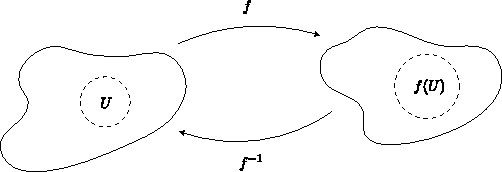
\includegraphics[scale=1.3]{fig/homeomorphism.pdf}
	\caption{A homeomorphism $f$.}
\end{figure}

\begin{defn}{Topological Property}{}
	A \textbf{topological property} is a property of topological space $X$ expressed entirely in terms of the topology on $X$ (the open sets of $X$).
\end{defn}

If $f:X \to Y$ is homeomorphic, then $Y$ has the topological properties of $X$. From this viewpoint, a homeomorphism is a bijective correspondence that preserves topological structure. This can be thought of as the topological analogue to isomorphisms in algebra.

\begin{defn}{Topological Embedding}{}
	Suppose $f: X \hookrightarrow Y$ is injective and continuous with $X,Y$ topological spaces. Let $Z$ be $f(X)$ as a subspace of $Y$, then $f':X \leftrightarrow Z$ (obtained by restricting the range of $f$) is bijective. If $f'$ is a homeomorphism of $X$ with $Z$, we say $f: X \hookrightarrow  Y$ is a \textbf{(topological) embedding} of $X$ in $Y$.
\end{defn}

{\color{red}Stuff about constructing continuous functions.}

\begin{thrm}{The Pasting Lemma}{}
	Let $X = A \cup B$, where $A$ and $B$ are closed in $X$ {\color{red}(something about this working for open sets too??)}. Let $f:A \to Y$ and $g:B\to Y$ be continuous. If $f(x)=g(x)$ for all $x \in A \cap B$, then $f$ and $g$ combine to give a continuous function $h : X \to Y$ by
	\[
		H(x)=
		\begin{cases}
			f(x) & x \in A \\
			g(x) & x\in B.
		\end{cases}
	\] 
\end{thrm}
\begin{proof}
	Let $C$ be closed in $Y$, then $h^{-1}(C) = f^{-1}(C) \cup g^{-1}(C)$. Since $f$ is continuous, $f^{-1}(C)$ is closed in $A$, so it is also closed in $X$. Similarly, $g^{-1}(C)$ is closed in $X$ as well. Then $h^{-1}(C)$ is the finite union of closed sets, so it is closed in $X$. Thus $h$ is continuous.

	Note that the condition $f(x) = g(x)$ for all $x \in A \cap B$ is not needed in this proof. It is only necessary to make $h$ an actual function.
\end{proof}

\begin{thrm}{Maps into Products}{}
	Define $f:A\to X \times Y$ by $f(a)=(f_1(a), f_2(a))$, for $f_1:A\to X$ and $f_2:A\to Y$. Then $f$ is continuous if and only if $f_1$ and $f_2$ are both continuous.
\end{thrm}
\begin{proof}
	Let $\pi_1:X\times Y\to X$ and $\pi_2:X\times Y\to Y$ be the obvious projections, which we know to be continuous.

	We begin with the forward implication. Suppose $f$ is continuous, then $f_1=\pi_1 \circ f$ and $f_2=\pi_2 \circ f$, so $f_1$ and $f_2$ are compositions of continuous functions. Thus they are both continuous themselves.

	Now we show the backward implication. Suppose $f_1$ and $f_2$ are continuous, then we'll show that for each basis element $U \times V$ of the topology on $X \times Y$, the preimage $f^{-1}(U \times V)$ is open. Take a point in the preimage $a \in f^{-1}(U \times V)$, then $f(a) \in U \times V$, so $f_1(a) \in U$ and $f_2(a) \in V$. Thus we have
	\[
		f^{-1}(U \times V) = f_1^{-1}(U) \cap f_2^{-1}(V).
	\] Since $U$ and $V$ are open and $f_1$ and $f_2$ are continuous, both of the sets in the above intersection are open. The finite intersection of open sets is open, so $f^{-1}(U\times V)$ is open, so $f$ is continuous.
\end{proof}

\begin{note}{}{}
	If $f:A\times B\to X$ instead, there is \textit{no} useful criterion for the continuity of $f$.
\end{note}


\end{document}
